%==============================================================================
\chapter{Introduction}
\label{chapter:intro}
%==============================================================================
One of the key features of Big Data is its complexity. 
We can define complexity in different ways.
It could be that data is coming from different sources, it could be the same data source representing different aspects of a resource, it could be different data sources representing the same property; this difference in representation, structure, or association makes it difficult to introduce common methodologies or algorithms to learn and predict from different types of data. 
The state of the art to handle this ambiguity and complexity of data is its representation or modeling using Semantic Web Technologies.

The Semantic Web Technologies follows a set of standards for the integration of data and information in addition to searching and querying it. 
To create such data, the information represented in unstructured form or referring to other structured or semi-structured representation is mapped to the \gls{RDF} data model. 
\gls{RDF} has a very flexible data model comprised of triples (subject, predicate, object), that can be interpreted as a labelled directed graph (s, p, o) with s and o being arbitrary resources (vertices) and p being the property (edge from s to o) among these two resources. 
Thus, a set of \gls{RDF} triples forms an inter-linkable graph whose flexibility allows to represent a large variety of highly to loosely structured datasets. 

\gls{RDF}, which was standardized by \gls{W3C}, is increasingly being adapted to model data in a variety of scenarios, partly due to the popularity of projects like linked open data and schema.org. 
This linked or semantically annotated data has grown steadily towards a massive scale\furl{http://lodstats.aksw.org/}.

Nevertheless, most existing solutions are limited to centralized environments only.
In order to deal with the massive data being produced at scale, the existing big data frameworks like Apache Spark\furl{http://spark.apache.org/} and Apache Flink\furl{https://flink.apache.org/} offer fault-tolerant, high available and scalable approaches to process this data efficiently. 
These frameworks have matured over recent years and offer a proven and reliable method for processing of large scale unstructured data.

In the past few years, MapReduce based, and related frameworks for Big Data processing have been explored for distributed processing of \gls{RDF} data as well. 
Some examples include the Spark-based S2RDF~\cite{Schatzle:2016:SRQ:2977797.2977806} which rewrites \gls{SPARQL} queries to SQL by using prior research by the RDB2RDF community and augments this approach by using precomputed semi-join tables. Approaches like SparkRDF~\cite{xu2015sparkrdf}, H2RDF~\cite{papailiou2013h} and H2RDF+~\cite{papailiou2012h2rdf} use triple dataset statistics to find best merge-join orders for efficient querying.
But, they are rather focused on one key element of the semantic stack, i.e. querying.
Therefore, there is a need for a comprehensive framework that offers capabilities of exploring, validating and querying a large amount of \gls{RDF} data at scale.
The main motivations behind using distributed computing are being able to handle data that does not fit on a single machine and achieve a speed-up and scalability.
Systems like \textit{Apache Spark} employ the \gls{BSP} synchronization approach, i.e. each parallel iteration/task has to wait for a synchronization step - all \textit{sub-tasks} must finish. 
This ensures correctness and fault tolerance.
However many applications, i.e. ranking resources (as PageRank is for web pages) are usually iteratively convergent in nature and this synchronization barrier at the end of each iteration overshadows the speed-up gained by distributed computation. 
In this thesis, we aim to exploit the existing communication, synchronization and distribution techniques to optimize the performance of Distributed Processing of \gls{RDF} Datasets when dealing with large amounts of data.

\section{Problem Definition and Challenges}
\label{sec:problem-definition-and-challenges}
Processing large-scale \gls{RDF} datasets is considered as one of the most challenging tasks in the Semantic Web~\cite{Benjamins02sixchallenges}.
The increase of the \gls{RDF} data in a rapid manner brings multiple challenges when exploring and getting more insight from the data.
More specifically, we face (i) a knowledge exploration problem, i.e. knowing the internal characteristics of the dataset. 
(ii) a data quality problem, i.e. which dataset is considered fit for use.
(iii) a processing challenge, i.e. can we retrieve and manage \gls{RDF} data when the size of the dataset increases.

In the following sections, we define the challenges that need to be addressed while designing a scalable and efficient processing framework for \gls{RDF} datasets.

\subsection{Challenge 1: Scalable Computation of RDF Dataset Statistics}
\label{sec:c1}
The first challenge to overcome when dealing with large-scale \gls{RDF} datasets is to have \textit{a priori} statistical information about its internal structure and coverage.
A significant fraction of RDF data available online\furl{https://lod-cloud.net/} today are stored as \gls{LOD}.
Large \gls{RDF} datasets, i.e. DBpeida~\cite{dbpedia-swj} are often collaborative and contain data that has been extracted semi-automatically or has been ingested from different sources.
Hence, such large-scale \gls{RDF} datasets do not have an apriori view of the data or a strict unified view for structuring the instances.
As a result, these processes derive noisily and, in a wrong case incomplete data~\cite{zaveri2015quality}.
In particular, for many applications such as data integration~\cite{michel:tel-01508602}, semantic search~\cite{Tonon2012CII}, interlinking~\cite{Dutta2014PAI}, or \gls{RDF} data partitioning do not take full advantage of the data without knowing the internal structure of the data.
In fact, there are already a number of tools, which offer such statistics, providing basic information about \gls{RDF} vocabularies~\cite{vandenbussche2015linked} and datasets~\cite{conf/dexaw/LangeggerW09,ermilov-2013-kesw}.
However, those efforts showed severe deficiencies in terms of performance when the dataset size goes beyond the main memory size of a single machine.
Therefore, to produce type information about large-scale \gls{RDF} datasets, we need a scalable computation of \gls{RDF} dataset statistics that is able to deal with massive \gls{RDF} datasets.

\subsection{Challenge 2: Quality Assessment of RDF Dataset at Scale}
\label{sec:c2}
Apart from knowing the internals of a given dataset, deciding how quality and what information is considered "\textit{fit for use}" is a challenge when the size of a dataset goes beyond the capacity of a single machine.
Assessing the quality of \gls{RDF} datasets is a crucial step to enhance the quality of the data being processed and published.
The process of assessing the quality of the data should be efficient and made available in order to facilitate the difference when it comes to finding the right information that is fit for use.
Some efforts have been made to provide a mechanism to assess the quality of the \gls{RDF} datasets~\cite{Debattista0AC18,farber2018,beek2018,debattista2016luzzu}.
However, these methods can either be used on a small portion of large datasets \cite{farber2018} or narrow down to specific problems e.g., syntactic accuracy of literal values~\cite{beek2018}, or accessibility of resources~\cite{Mihindukulasooriya2016LDSA}.
Existing efforts show severe deficiencies in terms of performance when data grows beyond the capabilities of a single machine.
This limits the applicability of existing solutions to medium-sized datasets only, in turn, paralyzing the role of applications in embracing the increasing volumes of the available datasets.

\subsection{Challenge 3: Efficient and Scalable SPARQL query evaluation}
\label{sec:c3}
More and more structured data is generated by an increasing number of organizations that are using \gls{RDF} as a model for data representation.
Therefore, analytics over such large-scale \gls{RDF} datasets lead us to a completely new level of computational complexity.
As a consequence, it becomes difficult to process such datasets using conventional approaches.
Many standalone \gls{SPARQL} query evaluators have been introduced in the past, nevertheless, as the volume of \gls{RDF} data increases, these single-machine solutions encounter performance bottlenecks in terms of data processing, loading, and querying.
For that reason, there is a need for a scalable and efficient framework that can handle large-scale \gls{RDF} datasets.
With that in mind, several approaches for distributed \gls{RDF} data processing have been proposed, e.g~\cite{sparqlgx-iswc-2016, Schatzle:2016:SRQ:2977797.2977806}.
We want to investigate and study implementations of current \gls{SPARQL} query evaluators through system-level characterizations and consequently propose our distributed approaches for \gls{RDF} data processing.

\subsection{Challenge 4: Adaptability of Exploiting large-scale RDF Datasets}
\label{sec:c4}
As the size of distributed systems for handling large-scale \gls{RDF} datasets grows, it becomes interestingly difficult to extract the right features from them.
Researchers have to deal with a very dynamic set of environments that these solutions are in contact with and it is becoming difficult to design a comprehensive framework that will be able to cater to all the user's needs in those settings.
In this thesis, we describe our approach with best practices, tools, and guidelines and show how it can be used (with some real use cases) to deploy and perform large-scale \gls{RDF} processing easily and efficiently.


\section{Research Questions}
\label{sec:research-questions}

As stated in the motivation section above and identified challenges, we define the main research question:

\begin{tcolorbox}
\centering
\textit{Is it possible to process large-scale \gls{RDF} datasets efficiently and effectively?}
\end{tcolorbox}

This research question then breaks down into four specific research questions.

Each challenge is mapped to specific research questions and altogether contribute to the overall research problem definition tackled throughout this thesis.

\begin{tcolorbox}
\textbf{\rqNr[RQ1]\label{rq:1}}: How can we efficiently explore the structure of the large-scale \gls{RDF} datasets?
\end{tcolorbox}

To address this question, we evaluate existing solutions that deal with statistical information of \gls{RDF} datasets.
In particular, we investigate the definitions proposed on~\cite{demter-2012-ekaw} and consider these 32 statistical criteria as a base for our system.
As our main goal is to offer a scalable and efficient approach for the statistical computation of large \gls{RDF} datasets, as an underlying engine, we consider one of the most prominent distributed frameworks, Apache Spark.
Finally, we study the use of novel distributed data structure representations -- known as \gls{RDD}~\cite{zaharia2012resilient}.
Within the scope of the thesis, we introduce a novel scalable approach for \gls{RDF} dataset statistics computation.
The results of the research question~\ref{rq:1} allow us to address the defined challenge (cf. Section~\ref{sec:c1}).

\begin{tcolorbox}
\textbf{\rqNr[RQ2]\label{rq:2}}: Can quality of large-scale \gls{RDF} datasets be assessed efficiently in a distributed manner?
\end{tcolorbox}

In order to answer this question, we investigate state-of-the-art quality assessment approaches with their metric definitions which can be used as a building block for quality measurements of \gls{RDF} datasets.
With the focus on the scalability, we derive quality metrics defined in~\cite{zaveri2015quality} and propose a scalable and efficient quality assessment framework that compute different quality metrics for large \gls{RDF} datasets.
Results obtained during the research question~\ref{rq:2} allow us to address the defined challenge (cf. Section~\ref{sec:c2}).

\begin{tcolorbox}
\textbf{\rqNr[RQ3]\label{rq:3}}: Can distributed \gls{RDF} datasets be queried efficiently and effectively?
\end{tcolorbox}

With the objective of answering this research question, we investigate different data storage representation and \gls{SPARQL} query evaluation and propose two different approaches for scalable and efficient \gls{RDF} data processing.
First, we introduce Sparklify: a scalable software component for efficient evaluation of \gls{SPARQL} queries over distributed \gls{RDF} datasets.
It uses SPARQL-to-SQL rewriter techniques for translating \gls{SPARQL} queries into Spark executable code.
The second approach we investigated and developed with the scope of this thesis is a scalable approach to evaluate \gls{SPARQL} queries over distributed \gls{RDF} datasets using a semantic-based partitioning.
It groups the facts based on the subject and its associated triples.
Results obtained during the research question~\ref{rq:3} allow us to address the defined challenge (cf. Section~\ref{sec:c3}). 
%Both approaches are implemented and integrated inside the state-of-the-art \gls{RDF} processing framework: SANSA.

\begin{tcolorbox}
\textbf{\rqNr[RQ4]\label{rq:4}}: How can we exploit large-scale \gls{RDF} datasets for a particular use case and ensure scalability?
\end{tcolorbox}

In response to this question, we present various use-cases and apply the techniques and approaches developed in this thesis.
Our findings show that the usage of distributed computing frameworks for large-scale \gls{RDF} analysis can provide a more adaptive and scalable solution for different use cases.

\section{Thesis Overview}
\label{sec:thesis-overview}
This section gives an overview of our main contributions conducted during this thesis and the research areas investigated.
References to scientific publications covering this study and an overview of the thesis outline are also covered.

\subsection{Contributions}
Our contributions cover a spectrum of research areas in the scope of distributed \gls{RDF} processing from the Scalable \gls{RDF} Datasets, \gls{RDF} Quality Assessment at Scale, and Scalable and Efficient \gls{SPARQL} evaluators, as depicted in Figure~\ref{fig:thesis-contributions}.

\begin{figure*}
\centering
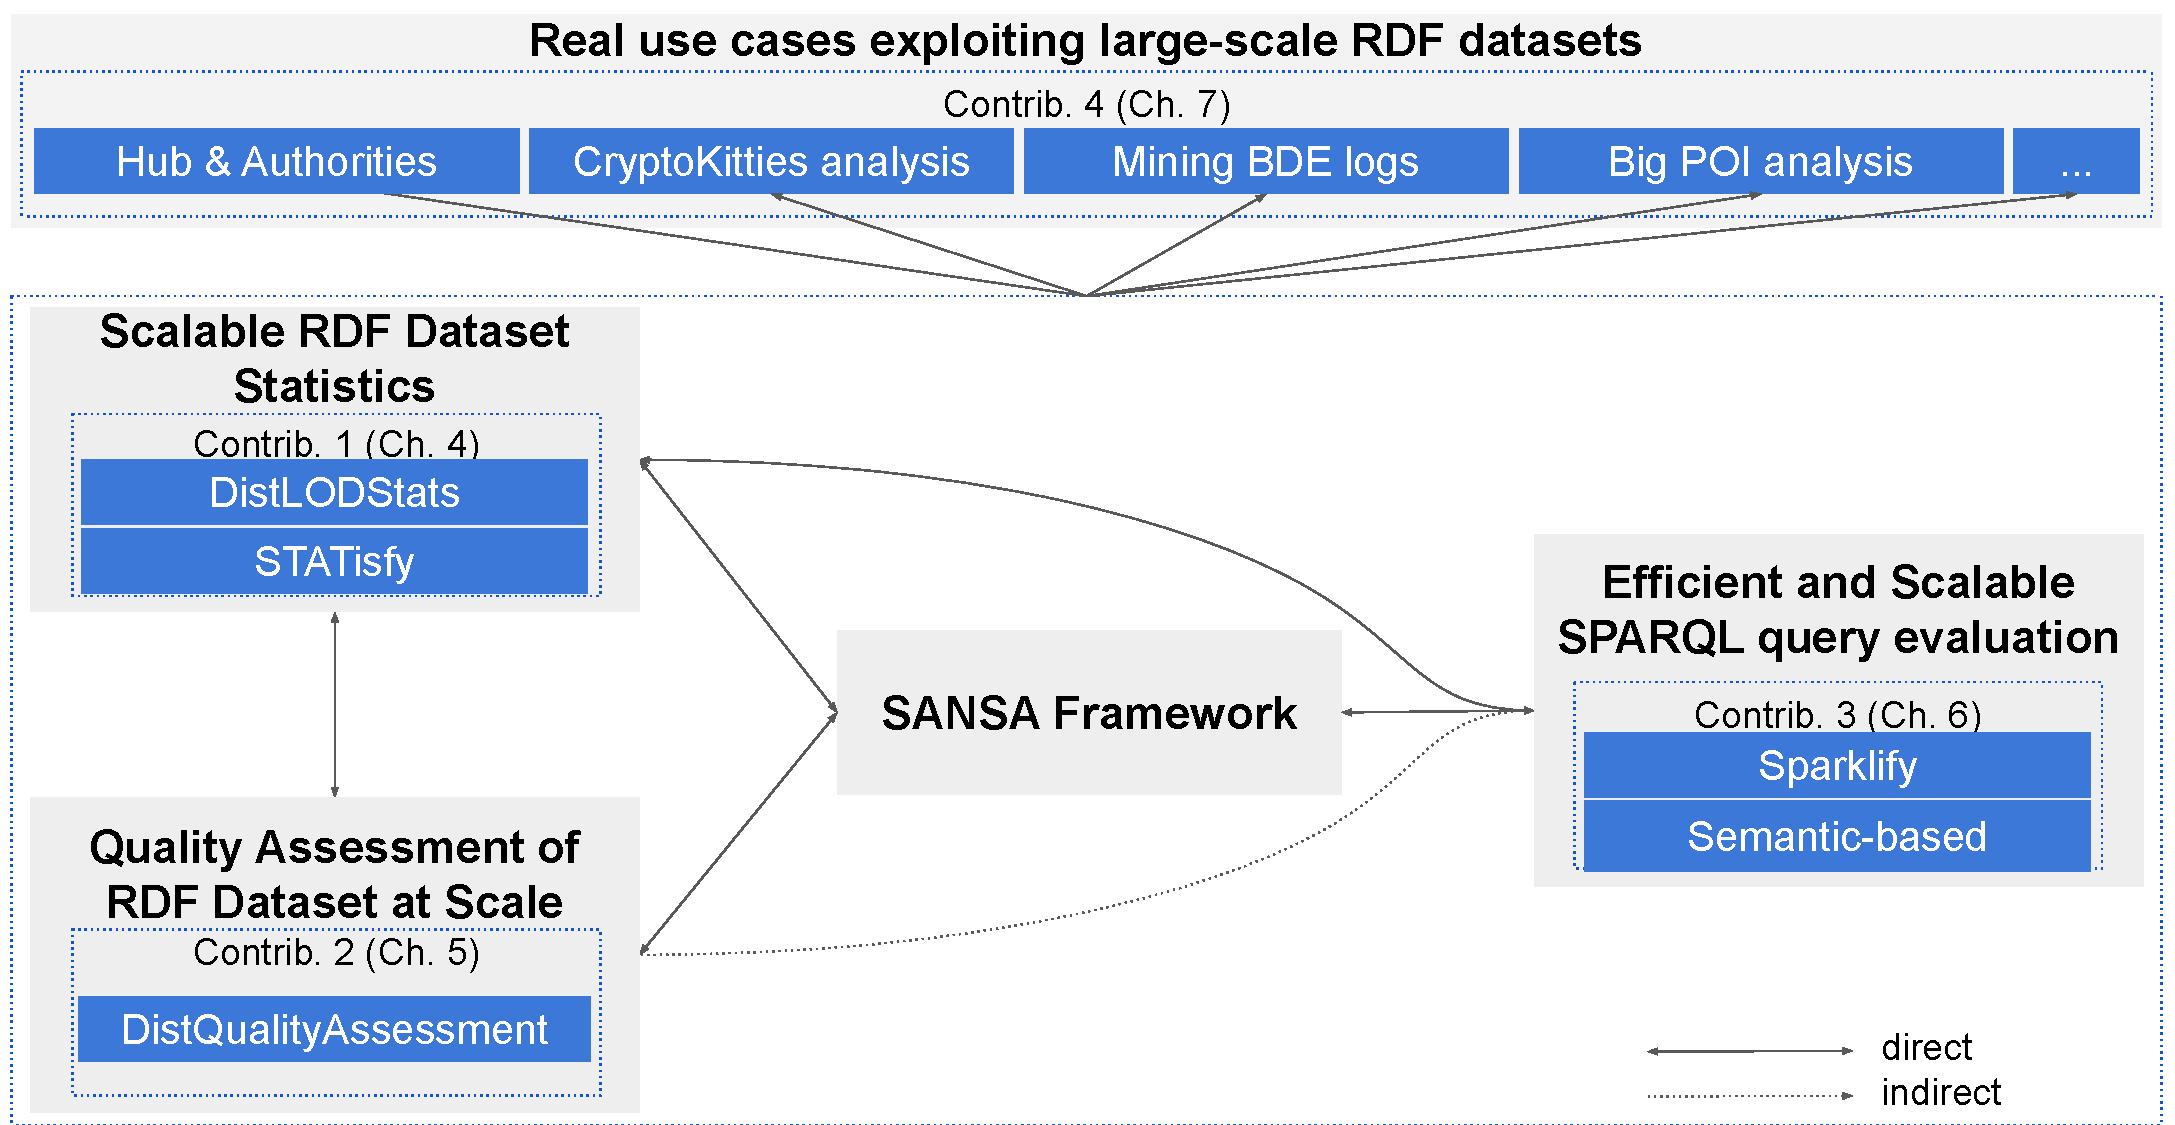
\includegraphics[width=1.0\columnwidth]{images/1_introduction/thesis-contributions.pdf}
\caption{\textbf{Thesis Contributions}. Four are the main contributions of this thesis: (1) a scalable distributed approach for evaluation of RDF dataset statistics; (2) a scalable framework for quality assessment of RDF datasets; (3) a scalable framework for SPARQL evaluation of large RDF data; (4) a comprehensive, open-source RDF processing and analytics stack for distributed in-memory computing with the real use cases where the thesis results are applicable.}
\label{fig:thesis-contributions}
\end{figure*}
%source: https://docs.google.com/presentation/d/1iacx2u1rCsCUb17GdTSpEitC6TwSuBFfD9s8yq7qWt4

\begin{enumerate}
    \item \textit{A Scalable Distributed Approach for Computation of \gls{RDF} Dataset Statistics}.
    
    For a better view and type of information when dealing with large-scale \gls{RDF} dataset we introduce DistLODStats, a software component for statistical calculations of large \gls{RDF} datasets, which scales out to clusters of machines.
    More specifically, we describe the first distributed in-memory approach for computing 32 different statistical criteria for \gls{RDF} datasets using Apache Spark.
    The preliminary results show that our distributed approach improves upon a previous centralized approach we compare against and provides approximately linear horizontal scale-up.
    The criteria are extensible beyond the 32 default criteria, is integrated into the larger SANSA framework and employed in at least four major usage scenarios beyond the SANSA community.
    More details on this contribution are provided in Chapter~\ref{chapter:dist_lod_stats}, and publications~\cite{sejdiu-2018-dist-lod-stats-iswc, sejdiu-2018-statisfy-iswc-poster}, which answer~\ref{rq:1}.
    
    \item \textit{A Scalable Framework for Quality Assessment of \gls{RDF} Datasets}.
    
    Quality of the data is one of the key components when designing and performing \gls{RDF} processing tasks.
    However, when dealing with large amounts of \gls{RDF} data, it becomes a challenge processing and exploring such quantitative and qualitative information.
    There exist a few approaches for the quality assessment of \gls{RDF} datasets, but their performance degrades with the increase in data size and quickly grows beyond the capabilities of a single machine. 
    To address this, we present DistQualityAssessment -- an open-source implementation of quality assessment of large \gls{RDF} datasets that can scale out to a cluster of machines.
    This is the first distributed, in-memory approach for computing different quality metrics for large \gls{RDF} datasets using Apache Spark. We also provide a quality assessment pattern that can be used to generate new scalable metrics that can be applied to big data.
    The work presented here is integrated with the SANSA framework and has been applied to at least three use cases beyond the SANSA community.   
    The results show that our approach is more generic, efficient, and scalable as compared to previously proposed approaches.
    See Chapter~\ref{chapter:dist_quality_assessment} for more information about this contribution, and publication~\cite{sejdiu-2019-sansa-dist-quality-assessment-iswc}.
    The DistQualityAssessment approach contributes to answering the research question~\ref{rq:2}.
    
    \item \textit{A Scalable Framework for \gls{SPARQL} evaluation of large \gls{RDF} data}.
    
    Over the last two decades, the amount of data that has been created, published and managed using Semantic Web standards and especially via \gls{RDF} has been increasing.
    As a result, the efficient processing of such big \gls{RDF} datasets has become challenging.
    Indeed, these processes require, both efficient storage strategies and query-processing engines, to be able to scale in terms of data size.
    In order to overcome this, we propose two different techniques that scale up to the cluster of machines.
    First, Sparklify: a scalable software component for efficient evaluation of \gls{SPARQL} queries over distributed \gls{RDF} datasets. It uses Sparqlify as a SPARQL-to-SQL rewriter for translating \gls{SPARQL} queries into Spark executable code.
    Our preliminary results demonstrate that Sparklify is more extensible, efficient, and scalable as compared to state-of-the-art approaches.
    Sparklify is integrated into a larger SANSA framework and it serves as a default query engine and has been used by at least three external use scenarios.
    The second approach we investigated and developed with the scope of this thesis is a scalable approach to evaluate \gls{SPARQL} queries over distributed \gls{RDF} datasets using a semantic-based partition and is implemented inside the state-of-the-art \gls{RDF} processing framework: SANSA.
    An evaluation of the performance of a semantic-based approach in processing large-scale \gls{RDF} datasets is also presented. 
    The preliminary results of the conducted experiments show that it can scale horizontally and perform well as compared with the previous Hadoop-based system.
    It is also comparable with the in-memory \gls{SPARQL} query evaluators when there is less shuffling involved.
    The Sparklify and semantic-based approaches contribute to answering the research question~\ref{rq:3}.
    A more detailed information on these contributions is given in Chapter~\ref{chapter:scalable_rdf_querying}, and publications~\cite{2019-sansa-sparklify-iswc, sejdiu-2019-sansa-semantic-based-semantics, sansa-sparklify-ISWC-demo}.
    
    \item \textit{A comprehensive, open-source \gls{RDF} processing and analytics stack for distributed in-memory computing.} 
    
    We collaborated with many different stockholders and research projects during the development of this thesis in order to solve the real-world scalable knowledge analysis and \gls{RDF} processing use cases.
    First, we mention here, Hub \& Authorities and CryptoKitties analysis use cases. 
    Alethio\furl{https://aleth.io/}, is an advanced analytics platform making Ethereum more accessible and digestible for everyone.
    Their extensive data set contains large-scale blockchain transaction data modelled in \gls{RDF} (currently encompassing more than 20B triples\furl{https://linkeddata.aleth.io/}) according to the structure of the Ethereum ontology~\cite{pfeffer2016ethon}.
    As the blockchain is evolving, many users want to know more about the important players of the chain. 
    With Hub \& Authorities' use case, we investigate and analyze the Ethereum blockchain network in order to identify the major entities across the transaction network. 
    By leveraging the rich data available through Alethio's platform in the form of \gls{RDF} triples we learn about the Hubs and Authorities of the Ethereum transaction network.
    Alethio uses our approach for efficient reading and processing of such large-scale \gls{RDF} data (transactions on Ethereum blockchain) in order to perform analytics e.g. finding top accounts, or typical behavior patterns of exchanges' deposit wallets and more.
    In another use case where Alethio is involved is the CryptoKitties analysis use case.
    CryptoKitties\furl{https://www.cryptokitties.co/} is one of the first games to be built on blockchain technology.
    Our solution empowers Alethio to read and query the data at scale for further analysis: game performance and customer behaviors.
    Within our solution, Alethio is able to get more insight from the CryptoKitties analyses, i.e the number of active users and the amount of spent Ether or correlation between indicators (e.g. to determine whether richer owners have the tendency to collect special/rare kitties which are more expensive).
    The second use case we were involved in was about mining BigDataEurope project logs.
    Big Data Europe (BDE)\furl{https://github.com/big-data-europe}~\cite{Auer+ICWE-2017} is an open-source big data processing platform allowing users to deploy Big Data processing tools and frameworks. 
    Those tools and frameworks usually generate large amounts of log data. 
    DistLODStats is used for computing statistics over those logs within the BDE platform. 
    BDE uses the Mu Swarm Logger service\furl{https://github.com/big-data-europe/mu-swarm-logger-service} for detecting docker events and convert their representation to \gls{RDF}. 
    In order to generate visualisations of log statistics, BDE then calls DistLODStats from SANSA-Notebooks~\cite{iermilov-2017-sansa-iswc-demo}.
    Finally, Big \gls{POI} analysis use case is developed.
    Among the various domains using large \gls{RDF} graphs, applications often rely on geographical information which is often represented via \gls{POI}s.
    In particular, one challenge is to extract patterns from \gls{POI} sets to discover \gls{AOI}s.
    To tackle this challenge, a typical method is to aggregate various points according to specific distances (e.g. geographical) via clustering algorithms. 
    In this study, we present a flexible architecture to design pipelines able to aggregate \gls{POI}s from contextual to geographical dimensions in a single run. 
    This solution allows any kind of clustering algorithm combinations to compute \gls{AOI}s and is built on top of a Semantic Web stack which allows multiple-source querying and filtering through \gls{SPARQL}.
    The architecture is embedded inside a state-of-the-art Semantic Web stack, SANSA, and then benefits from the advantages of it.
    The best practices, guidelines, easy to deploy and use in a lightweight allows us to quickly adapt the SANSA framework from the semantic web community and other fields of data science, thus allowing us to answer research question~\ref{rq:4}.
    Some of the use cases are described in Chapter~\ref{chapter:implementation_and_use_cases}, and publications~\cite{lehmann-2017-sansa-iswc, iermilov-2017-sansa-iswc-demo, sansa-hubs-and-authorities-transaction-semantics19-poster, piping-clustering-eswc19-poster, graux-2018-sansa-ethereum-semantics-poster, Auer+ICWE-2017}.

\end{enumerate}


\subsection{List of Publications}
In this thesis, part of the work is based on the following publications~\cite{sejdiu-2019-sansa-dist-quality-assessment-iswc, 2019-sansa-sparklify-iswc, sejdiu-2019-sansa-semantic-based-semantics, sejdiu-2018-dist-lod-stats-iswc, lehmann-2017-sansa-iswc, Auer+ICWE-2017, sansa-sparklify-ISWC-demo, sansa-hubs-and-authorities-transaction-semantics19-poster, piping-clustering-eswc19-poster, sejdiu-2018-statisfy-iswc-poster, graux-2018-sansa-ethereum-semantics-poster, iermilov-2017-sansa-iswc-demo, KESW_2017_BDE}:
\begin{itemize}
\item \emph{Conference Papers (peer reviewed)}
\begin{enumerate}
    
    \item \textbf{Gezim Sejdiu}; Anisa Rula; Jens Lehmann; and Hajira Jabeen, “\href{http://jens-lehmann.org/files/2019/iswc_dist_quality_assessment.pdf}{A Scalable Framework for Quality Assessment of RDF Datasets},” in Proceedings of 18th International Semantic Web Conference (ISWC), 2019. \texttt{URL}:~\url{http://jens-lehmann.org/files/2019/iswc_dist_quality_assessment.pdf}

    \item Claus Stadler; \textbf{Gezim Sejdiu}; Damien Graux; and Jens Lehmann, “\href{http://jens-lehmann.org/files/2019/iswc_sparklify.pdf}{Sparklify: A Scalable Software Component for Efficient evaluation of SPARQL queries over distributed RDF datasets},” in Proceedings of 18th International Semantic Web Conference (ISWC), 2019. \texttt{URL}:~\url{http://jens-lehmann.org/files/2019/iswc_sparklify.pdf}
    This article is a joint work with Claus Stadler, a PhD student at the University of Leipzig. 
    In this article, I devised the implementation of the conceptual architecture, helped on the implementation of the proposed approach, reviewed related work, and prepared of the experiments and analysis of the obtained results.

    \item \textbf{Gezim Sejdiu}; Damien Graux; Imran Khan; Ioanna Lytra; Hajira Jabeen; and Jens Lehmann, “\href{https://gezimsejdiu.github.io/publications/semantic_based_query_paper_SEMANTICS2019.pdf}{Towards A Scalable Semantic-based Distributed Approach for SPARQL query evaluation},” 15th International Conference on Semantic Systems (SEMANTiCS), Research \& Innovation , 2019. \texttt{URL}:~\url{https://gezimsejdiu.github.io/publications/semantic_based_query_paper_SEMANTICS2019.pdf}

    \item \textbf{Gezim Sejdiu}; Ivan Ermilov; Jens Lehmann; and Mohamed Nadjib-Mami, “\href{http://jens-lehmann.org/files/2018/iswc_distlodstats.pdf}{DistLODStats: Distributed Computation of RDF Dataset Statistics},” in Proceedings of 17th International Semantic Web Conference (ISWC), 2018. \texttt{URL}:~\url{http://jens-lehmann.org/files/2018/iswc_distlodstats.pdf}

    \item Jens Lehmann; \textbf{Gezim Sejdiu}; Lorenz Bühmann; Patrick Westphal; Claus Stadler; Ivan Ermilov; Simon Bin; Nilesh Chakraborty; Muhammad Saleem; Axel-Cyrille Ngomo Ngonga; and Hajira Jabeen, “\href{http://svn.aksw.org/papers/2017/ISWC_SANSA_SoftwareFramework/public.pdf}{Distributed Semantic Analytics using the SANSA Stack},”; in Proceedings of 16th International Semantic Web Conference - Resources Track (ISWC’2017), 2017. \texttt{URL}:~\url{http://svn.aksw.org/papers/2017/ISWC_SANSA_SoftwareFramework/public.pdf}
    
    \item Ivan Ermilov; Axel-Cyrille Ngonga Ngomo; Aad Versteden; Hajira Jabeen; \textbf{Gezim Sejdiu}; Giorgos Argyriou; Luigi Selmi; Jürgen Jakobitsch; and Jens Lehmann, “\href{https://svn.aksw.org/papers/2017/KESW_BDE_Workflow/public.pdf}{Managing Lifecycle of Big Data Applications},”; in KESW, 2017. \texttt{URL}:~\url{https://svn.aksw.org/papers/2017/KESW_BDE_Workflow/public.pdf}
    This article is a joint work with Ivan Ermilov, a PhD student at the University of Leipzig. 
    In this article, I helped with the implementation of the proposed approach and SC4 (Transport) use case, reviewed related work, and preparation of the experiments and analysis of the obtained results.

    \item Sören Auer; Simon Scerri; Aad Versteden; Erika Pauwels; Angelos Charalambidis; Stasinos Konstantopoulos; Jens Lehmann; Hajira Jabeen; Ivan Ermilov; \textbf{Gezim Sejdiu}; Andreas Ikonomopoulos; Spyros Andronopoulos; Mandy Vlachogiannis; Charalambos Pappas; Athanasios Davettas; Iraklis A. Klampanos; Efstathios Grigoropoulos; Vangelis Karkaletsis; Victor Boer; Ronald Siebes; Mohamed Nadjib Mami; Sergio Albani; Michele Lazzarini; Paulo Nunes; Emanuele Angiuli; Nikiforos Pittaras; George Giannakopoulos; Giorgos Argyriou; George Stamoulis; George Papadakis; Manolis Koubarakis; Pythagoras Karampiperis; Axel-Cyrille Ngonga Ngomo; and Maria-Esther Vidal, “\href{http://jens-lehmann.org/files/2017/icwe_bde.pdf}{The BigDataEurope Platform – Supporting the Variety Dimension of Big Data},” in 17th International Conference on Web Engineering (ICWE2017), 2017. \texttt{URL}:~\url{http://jens-lehmann.org/files/2017/icwe_bde.pdf}
    This article is a joint work with the BDE consortium. 
    In this article, I contributed within the semantic layer, more specifically; bringing the Big Data Analytics for \gls{RDF} into the BDE platform and co-contributing into dockerizing BDE components.
     
\end{enumerate}
    \item \emph{Demo \& Poster Papers (peer reviewed)}
    \begin{enumerate}
    \setcounter{enumi}{7}

    \item Claus Stadler; \textbf{Gezim Sejdiu}; Damien Graux; and Jens Lehmann. "\href{https://gezimsejdiu.github.io/publications/sansa-sparklify-ISWC-demo.pdf}{Querying large-scale RDF datasets using the SANSA framework}".  In Proceedings of 18th International Semantic Web Conference (ISWC), Poster \& Demos, 2019. \texttt{URL}:~\url{https://gezimsejdiu.github.io/publications/sansa-sparklify-ISWC-demo.pdf}
    This demonstration article is a joint work with Claus Stadler, a PhD student at the University of Leipzig.
    In this article, I helped in describing the architecture and implementation of the running example.

    \item Danning Sui; \textbf{Gezim Sejdiu}; Damien Graux; and Jens Lehmann. "\href{https://gezimsejdiu.github.io/publications/sansa-hubs-and-authorities-transaction-semantics19-poster.pdf}{The Hubs and Authorities Transaction NetworkAnalysis using the SANSA framework}".  In 15th International Conference on Semantic Systems (SEMANTiCS), Poster \& Demos, 2019. \texttt{URL}:~\url{http://tiny.cc/4ukxcz}
    
    \item Rajjat Dadwal; Damien Graux; \textbf{Gezim Sejdiu}; Hajira Jabeen; and Jens Lehmann. "\href{https://gezimsejdiu.github.io/publications/piping-clustering-eswc19-poster.pdf}{Clustering Pipelines of large RDF POI Data}" in Proceedings of 16th Extended Semantic Web Conference (ESWC), Poster \& Demos, 2019. \texttt{URL}:~\url{https://gezimsejdiu.github.io/publications/piping-clustering-eswc19-poster.pdf}
    
    \item \textbf{Gezim Sejdiu}; Ivan Ermilov; Jens Lehmann; and Mohamed-Nadjib Mami, “\href{http://jens-lehmann.org/files/2018/iswc_statisfy_pd.pdf}{STATisfy Me: What are my Stats?},” in Proceedings of 17th International Semantic Web Conference (ISWC), Poster \& Demos, 2018. \texttt{URL}:~\url{http://jens-lehmann.org/files/2018/iswc_statisfy_pd.pdf}
    
    \item Damien Graux; \textbf{Gezim Sejdiu}; Hajira Jabeen; Jens Lehmann; Danning Sui; Dominik Muhs; and Johannes Pfeffer, “\href{http://jens-lehmann.org/files/2018/semantics_ethereum_pd.pdf}{Profiting from Kitties on Ethereum: Leveraging Blockchain RDF with SANSA},” in 14th International Conference on Semantic Systems, Poster \& Demos, 2018. \texttt{URL}:~\url{http://jens-lehmann.org/files/2018/semantics_ethereum_pd.pdf}
    
    \item Ivan Ermilov; Jens Lehmann; \textbf{Gezim Sejdiu}; Lorenz Bühmann; Patrick Westphal; Claus Stadler; Simon Bin; Nilesh Chakraborty; Henning Petzka; Muhammad Saleem; Axel-Cyrille Ngomo Ngonga; and Hajira Jabeen, “\href{http://jens-lehmann.org/files/2017/iswc_pd_sansa.pdf}{The Tale of Sansa Spark},” in Proceedings of 16th International Semantic Web Conference, Poster \& Demos, 2017 ({\color{darkred}\textbf{Best Demo Award}}). \texttt{URL}:~\url{http://jens-lehmann.org/files/2017/iswc_pd_sansa.pdf}
    This demonstration article is joint work with Ivan Ermilov, a PhD student at the University of Leipzig. 
    In this article, I helped in describing the architecture, implementation of the examples and demonstration of the prototype.
        
    \end{enumerate}
\end{itemize}

Appendix~\ref{sec:appendix-publications} contains the complete list of publications finished during the PhD studies.

\section{Thesis Outline}
\label{sec:thesis-outline}
The thesis consists of eight chapters.
%and is structured as follows:
Chapter~\ref{chapter:intro} introduces the thesis starting with the main research problem and challenges, motivation, research questions, scientific contributions addressing research questions, and a list of published scientific papers describing these contributions.
Chapter~\ref{chapter:preliminaries} presents basic concepts and background about Semantic Web technologies and the Hadoop Ecosystem for a comprehensive overview of the research problem. 
Chapter~\ref{chapter:related} describes state-of-the-art efforts in the field of processing \gls{RDF} datasets w.r.t research problem.
We provide an overview of existing \gls{RDF} dataset statistics systems, quality assessment systems, and \gls{SPARQL} query evaluators in order to provide a thorough knowledge of their limitations, and the identified gaps we cover in this thesis.
In Chapter~\ref{chapter:dist_lod_stats} we introduce a scalable approach for the statistical calculation of large \gls{RDF} datasets, which scales out to a cluster of machines.
More specifically, we describe the first distributed in-memory approach for computing 32 different statistical criteria for \gls{RDF} dataset using the Apache Spark framework.
Chapter~\ref{chapter:dist_quality_assessment} introduces a scalable approach for quality assessment of \gls{RDF} datasets.
The presented approach offers generic features to solve common data quality checks.
As a consequence, this can enable further applications to build trusted data utilities.
We have demonstrated empirically that our approach improves upon the previous centralized approach that we have compared against.
We also provide a quality assessment pattern that can be used to generate new scalable metrics that can be applied to big data.
Chapter~\ref{chapter:scalable_rdf_querying} proposes two storage strategies and query engine implementations for efficient and scalable querying and processing \gls{RDF} datasets.
First, Sparklify: a scalable software component for efficient evaluation of \gls{SPARQL} queries over distributed \gls{RDF} datasets. 
It uses a SPARQL-to-SQL rewriter technique for translating \gls{SPARQL} queries into Spark executable code.
The second approach we investigated and developed with the scope of this thesis is a scalable approach to evaluate \gls{SPARQL} queries over distributed \gls{RDF} datasets using a semantic-based partition.
Moreover, in this chapter, we present the evaluations of our implementations as compared with state of the art \gls{SPARQL} query evaluators.
Chapter~\ref{chapter:implementation_and_use_cases} presents real world use-cases powered by our solutions. 
More specifically, we show the usage of SANSA in general and the solutions proposed during this work in order to answer the research problem~\ref{rq:4}, and, consequently, validate the solutions proposed for the problems~\ref{rq:1}, \ref{rq:2}, and \ref{rq:3}.
Chapter~\ref{chapter:conclusion} conclude the thesis with an overall overview of the contributions made during this research work and a discussion on the future work based on the limitations of the actual solutions. 
